%!TeX root=../wowtop.tex

\ArtChapter[The \emph{Thunder Child}]{17head}

\lettrine[lines=4,findent=2pt]{H}{ad} the Martians aimed only at destruction, they might on Monday have annihilated the entire population of London, as it spread itself slowly through the home counties. Not only along the road through Barnet, but also through Edgware and Waltham Abbey, and along the roads eastward to Southend and Shoeburyness, and south of the Thames to Deal and Broadstairs, poured the same frantic rout. If one could have hung that June morning in a balloon in the blazing blue above London every northward and eastward road running out of the tangled maze of streets would have seemed stippled black with the streaming fugitives, each dot a human agony of terror and physical distress. I have set forth at length in the last chapter my brother's account of the road through Chipping Barnet, in order that my readers may realise how that swarming of black dots appeared to one of those concerned. Never before in the history of the world had such a mass of human beings moved and suffered together. The legendary hosts of Goths and Huns, the hugest armies Asia has ever seen, would have been but a drop in that current. And this was no disciplined march; it was a stampede—a stampede gigantic and terrible—without order and without a goal, six million people unarmed and unprovisioned, driving headlong. It was the beginning of the rout of civilisation, of the massacre of mankind.

Directly below him the balloonist would have seen the network of streets far and wide, houses, churches, squares, crescents, gardens—already derelict—spread out like a huge map, and in the southward \textit{blotted}. Over Ealing, Richmond, Wimbledon, it would have seemed as if some monstrous pen had flung ink upon the chart. Steadily, incessantly, each black splash grew and spread, shooting out ramifications this way and that, now banking itself against rising ground, now pouring swiftly over a crest into a new-found valley, exactly as a gout of ink would spread itself upon blotting paper.

\begin{letter}
	\begin{figure}[tb!]
	\centering
	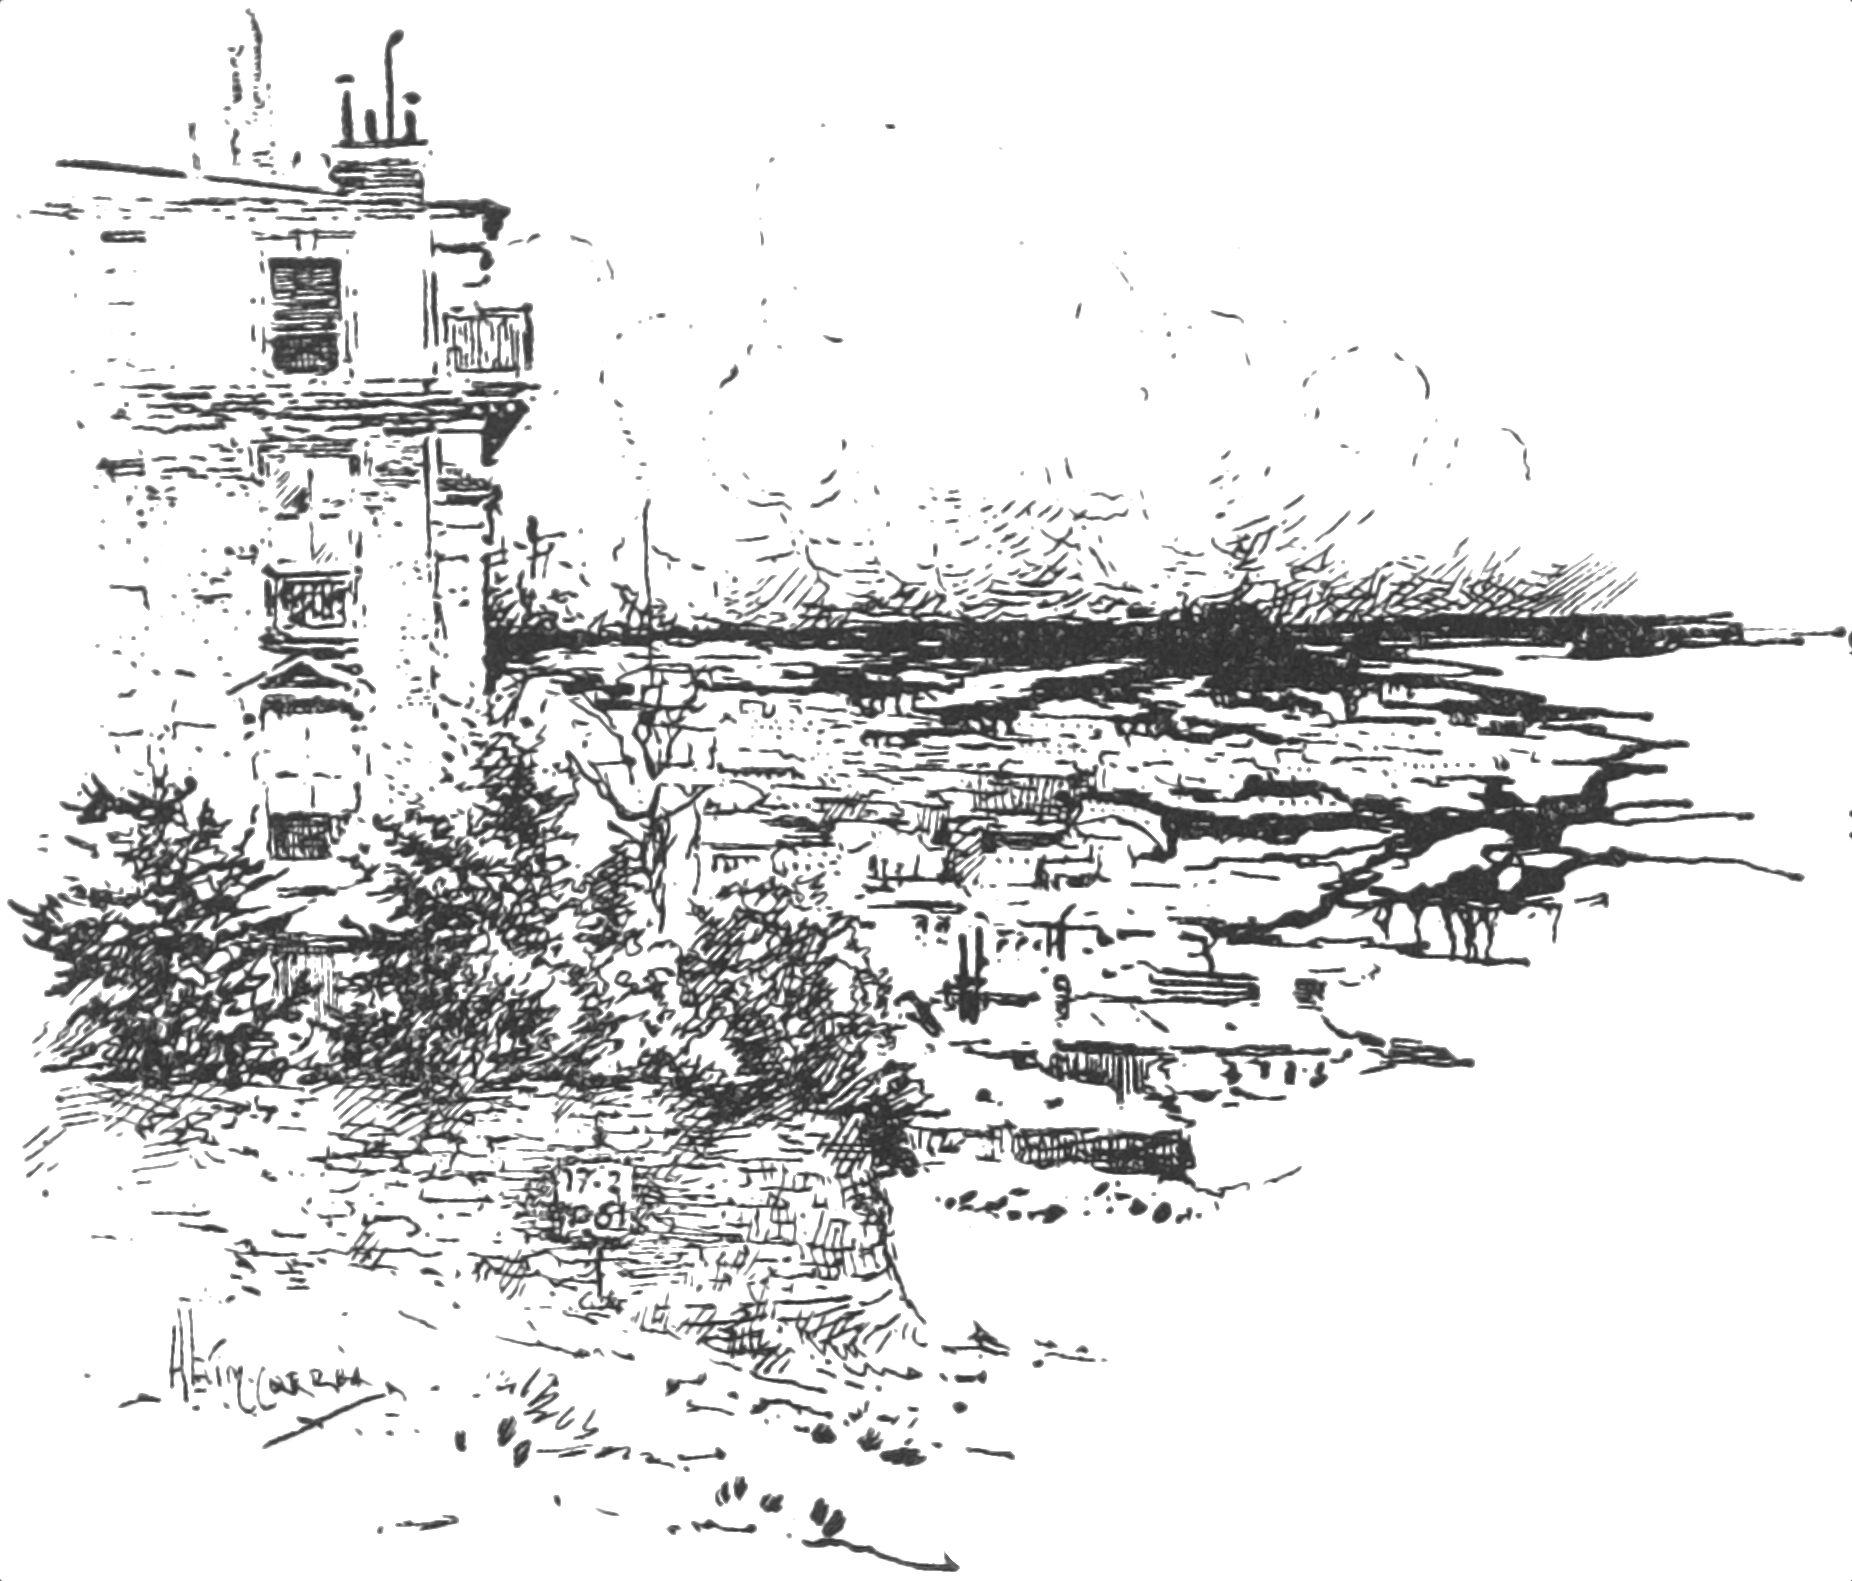
\includegraphics[width=\textwidth]{17hillview}
	\end{figure}
\end{letter}

\begin{a4}
	\begin{figure}[tb!]
	\centering
	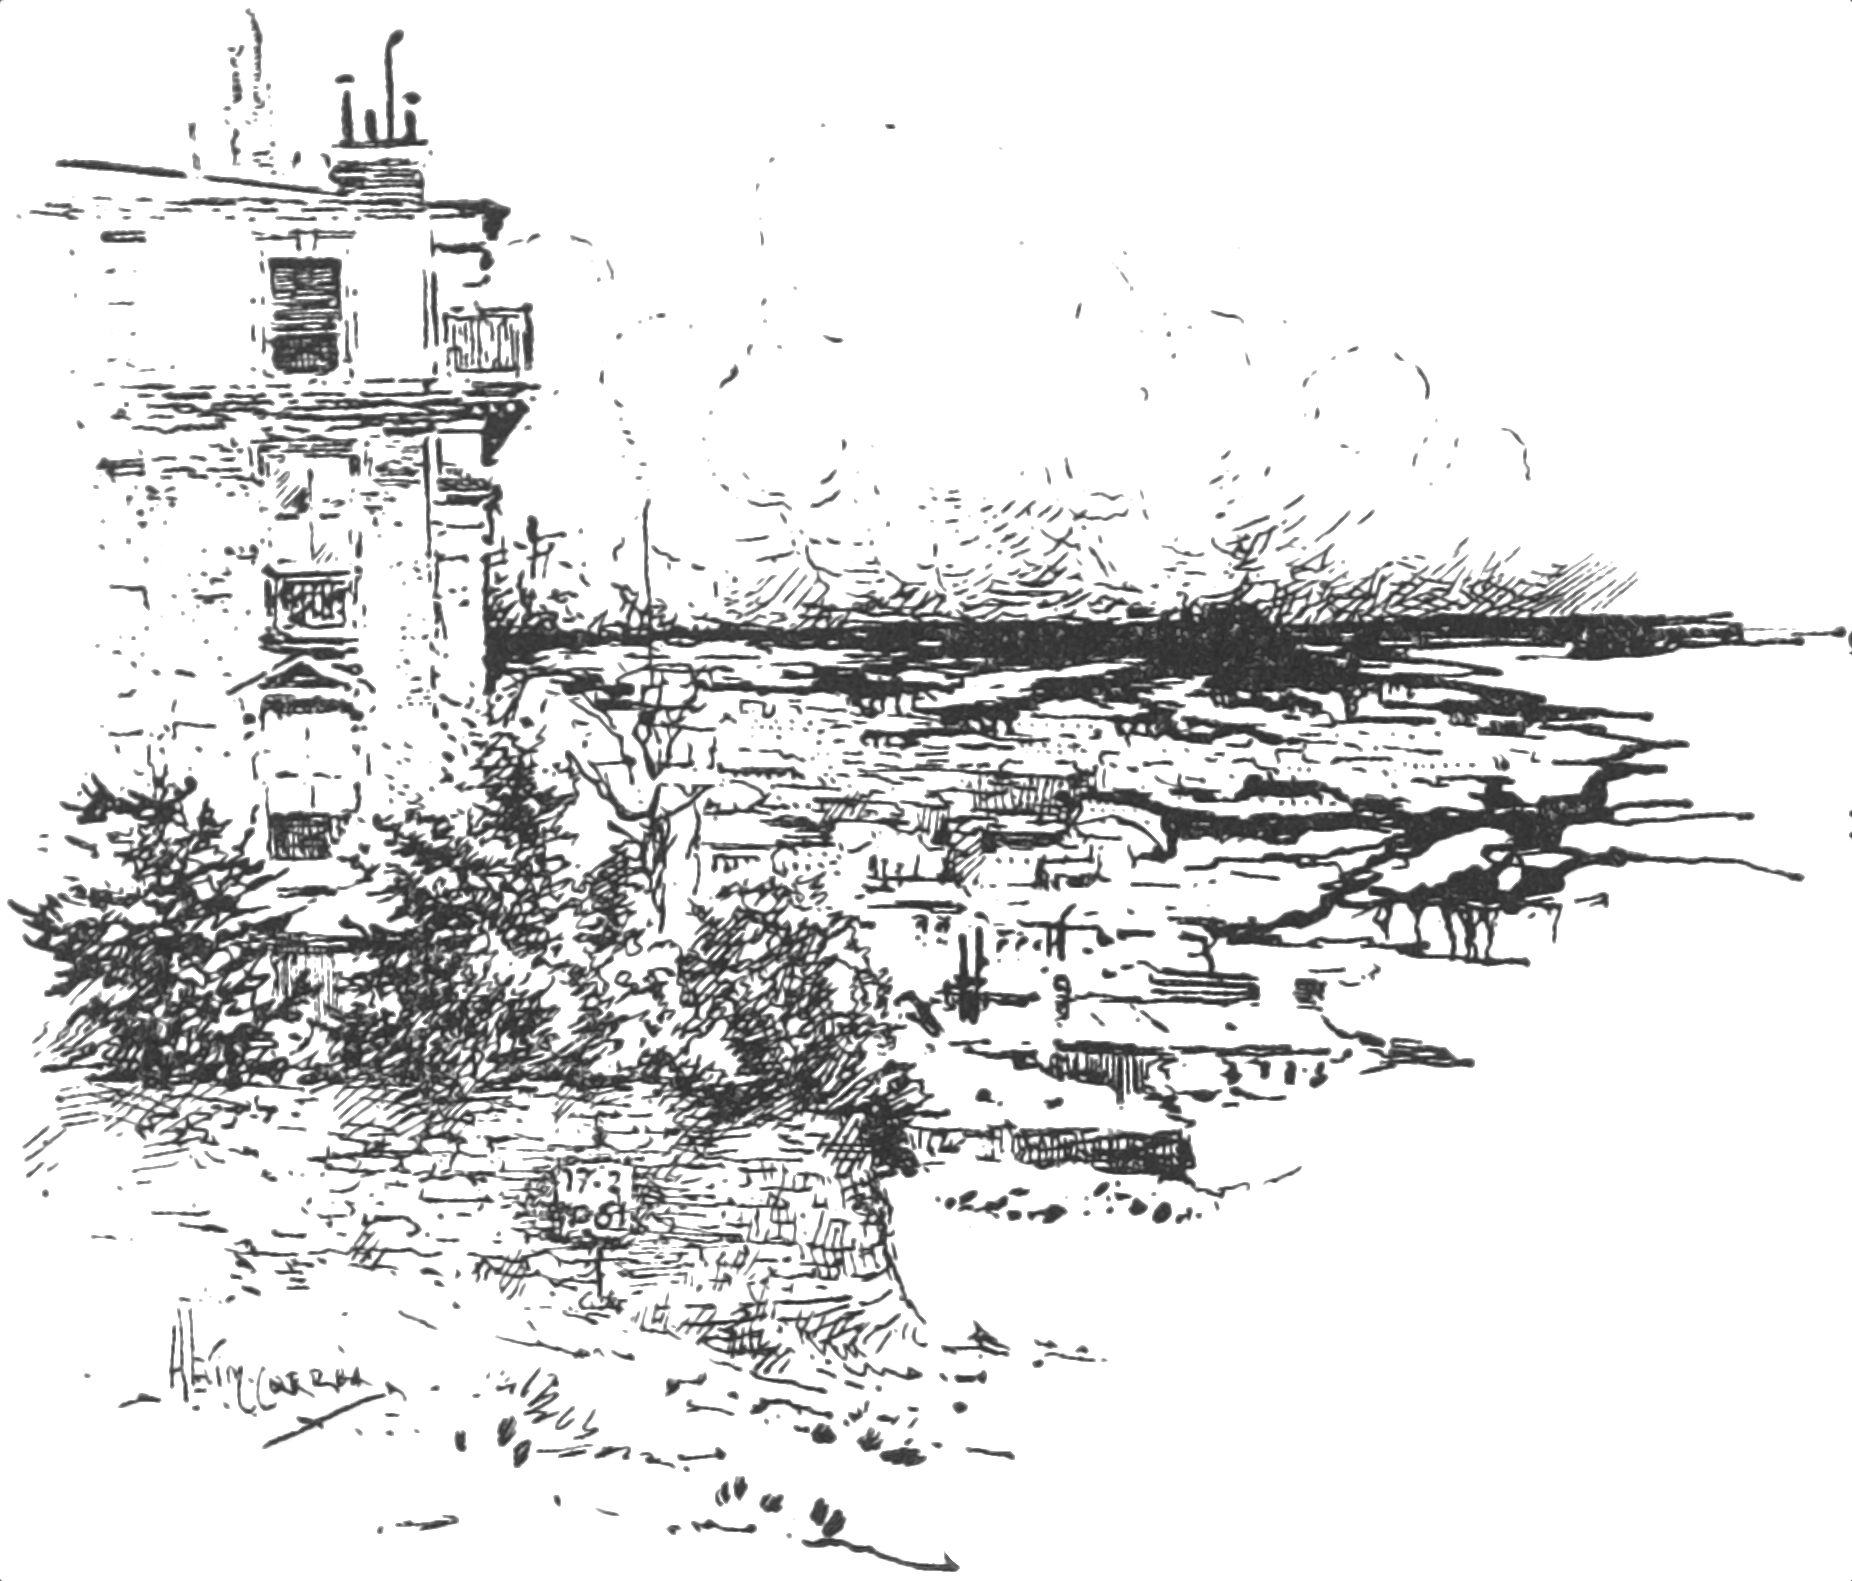
\includegraphics[width=.9\textwidth]{17hillview}
	\end{figure}
\end{a4}

%\begin{wrapfigure}{O}{0.6\textwidth}
%\centering
%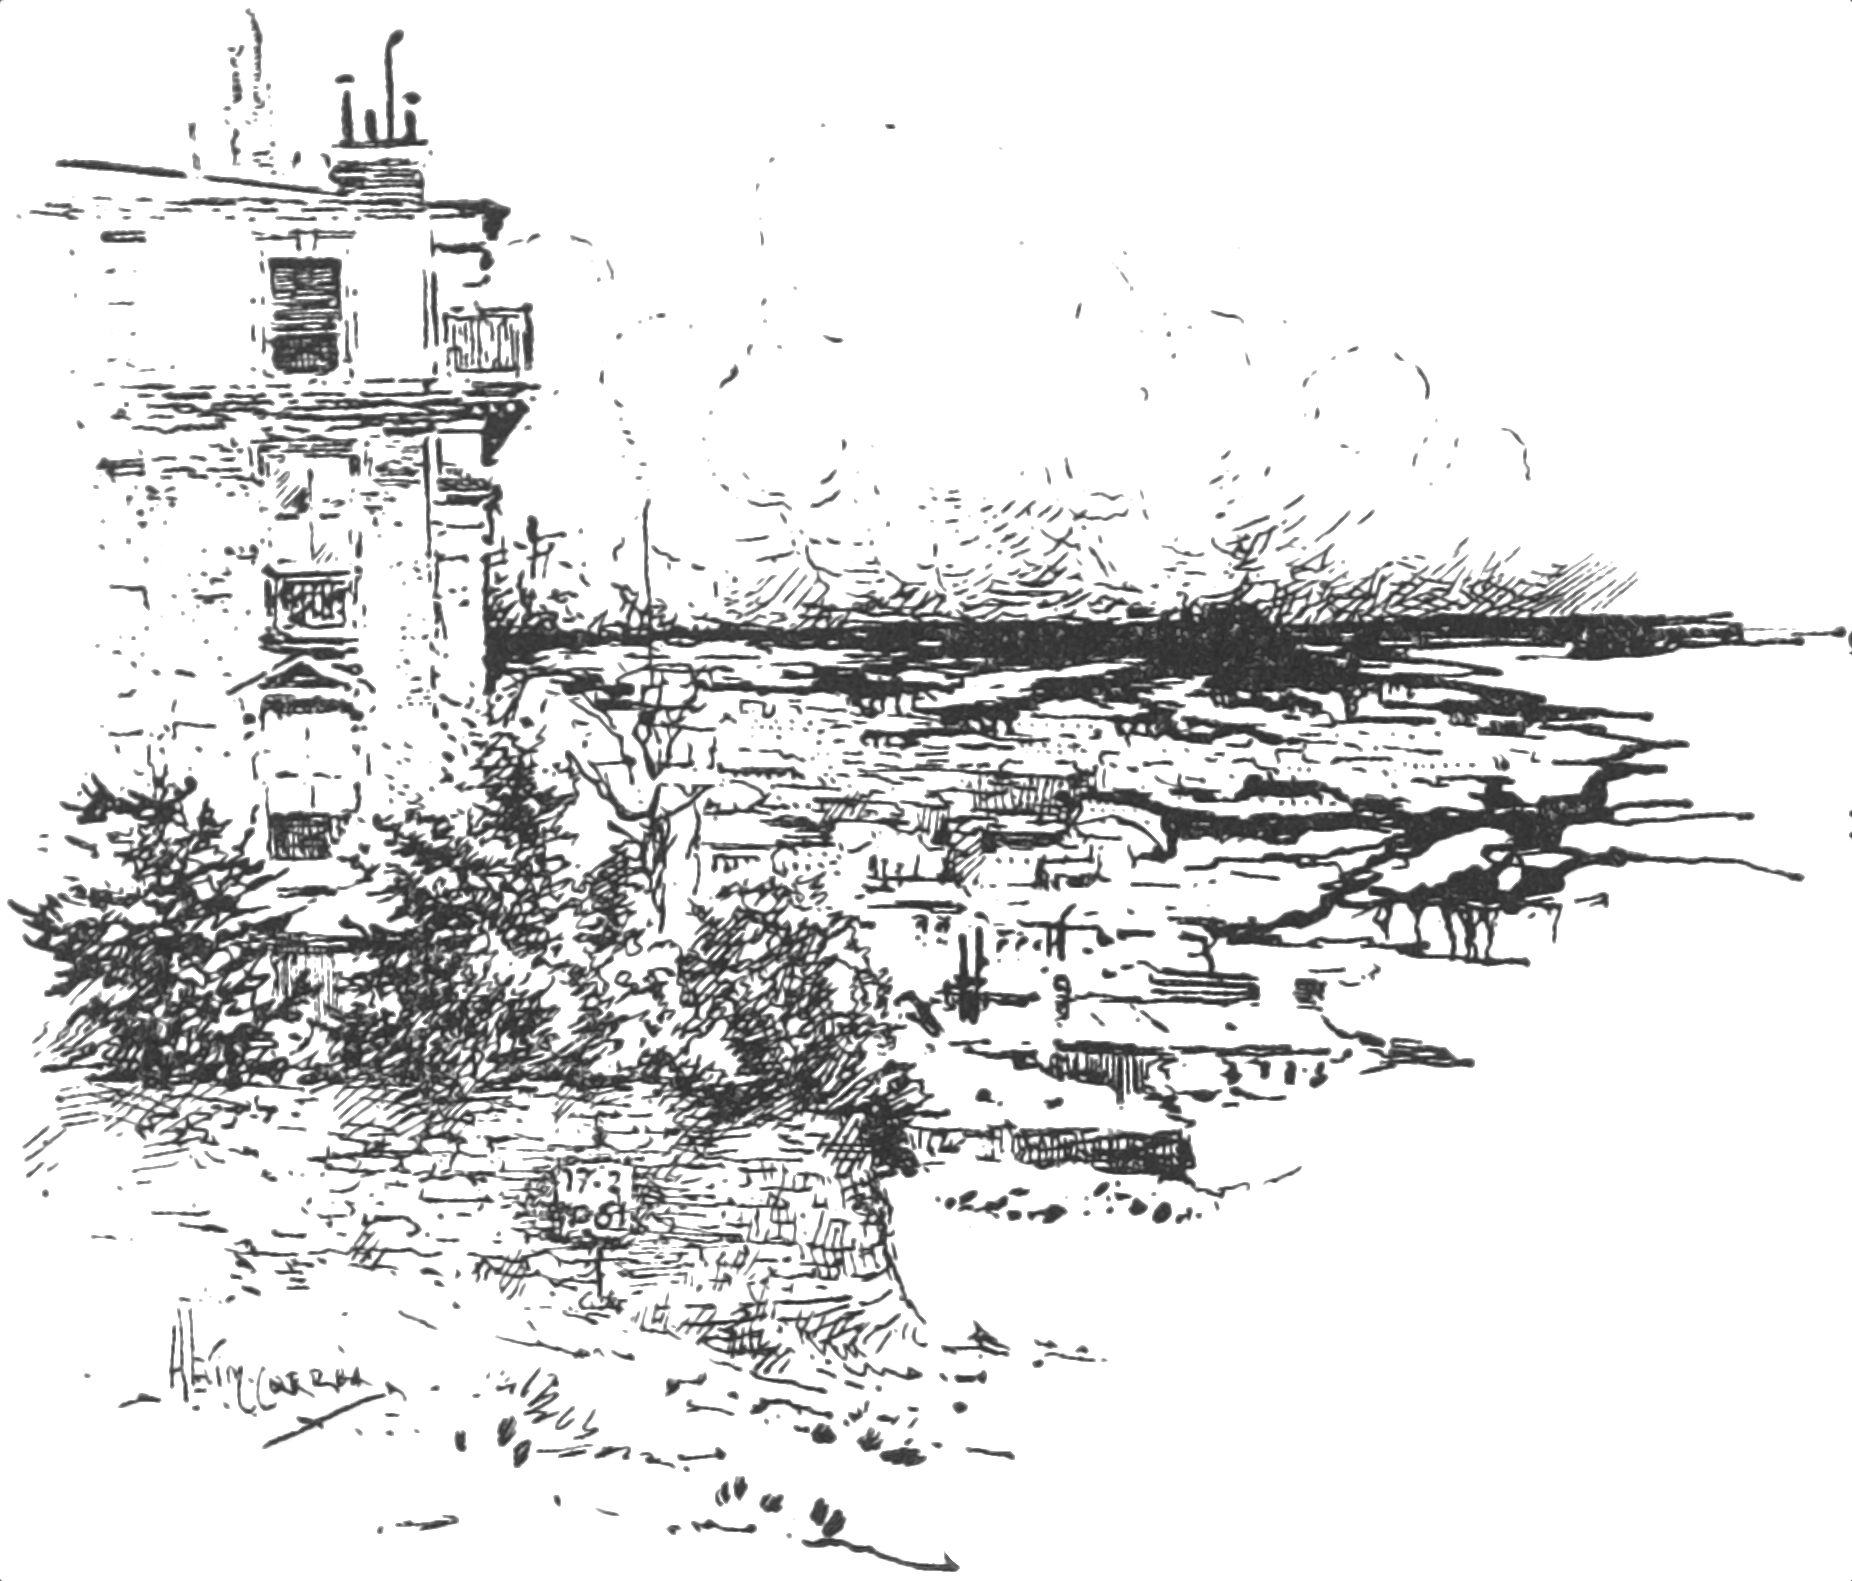
\includegraphics[width=0.6\textwidth]{17hillview}
%\end{wrapfigure}

And beyond, over the blue hills that rise southward of the river, the glittering Martians went to and fro, calmly and methodically spreading their poi\-son cloud over this patch of country and then over that, laying it again with their steam jets when it had served its purpose, and taking possession of the conquered country. They do not seem to have aimed at extermination so much as at complete demoralisation and the destruction of any opposition. They exploded any stores of powder they came upon, cut every telegraph, and wrecked the railways here and there. They were hamstringing mankind. They seemed in no hurry to extend the field of their operations, and did not come beyond the central part of London all that day. It is possible that a very considerable number of people in London stuck to their houses through Monday morning. Certain it is that many died at home suffocated by the Black Smoke.

Until about midday the Pool of London was an astonishing scene. Steamboats and shipping of all sorts lay there, tempted by the enormous sums of money offered by fugitives, and it is said that many who swam out to these vessels were thrust off with boathooks and drowned. About one o'clock in the afternoon the thinning remnant of a cloud of the black vapour appeared between the arches of Blackfriars Bridge. At that the Pool became a scene of mad confusion, fighting, and collision, and for some time a multitude of boats and barges jammed in the northern arch of the Tower Bridge, and the sailors and lightermen had to fight savagely against the people who swarmed upon them from the riverfront. People were actually clambering down the piers of the bridge from above.

When, an hour later, a Martian appeared beyond the Clock Tower and waded down the river, nothing but wreckage floated above Limehouse.

\begin{figure}[tb!]
\centering
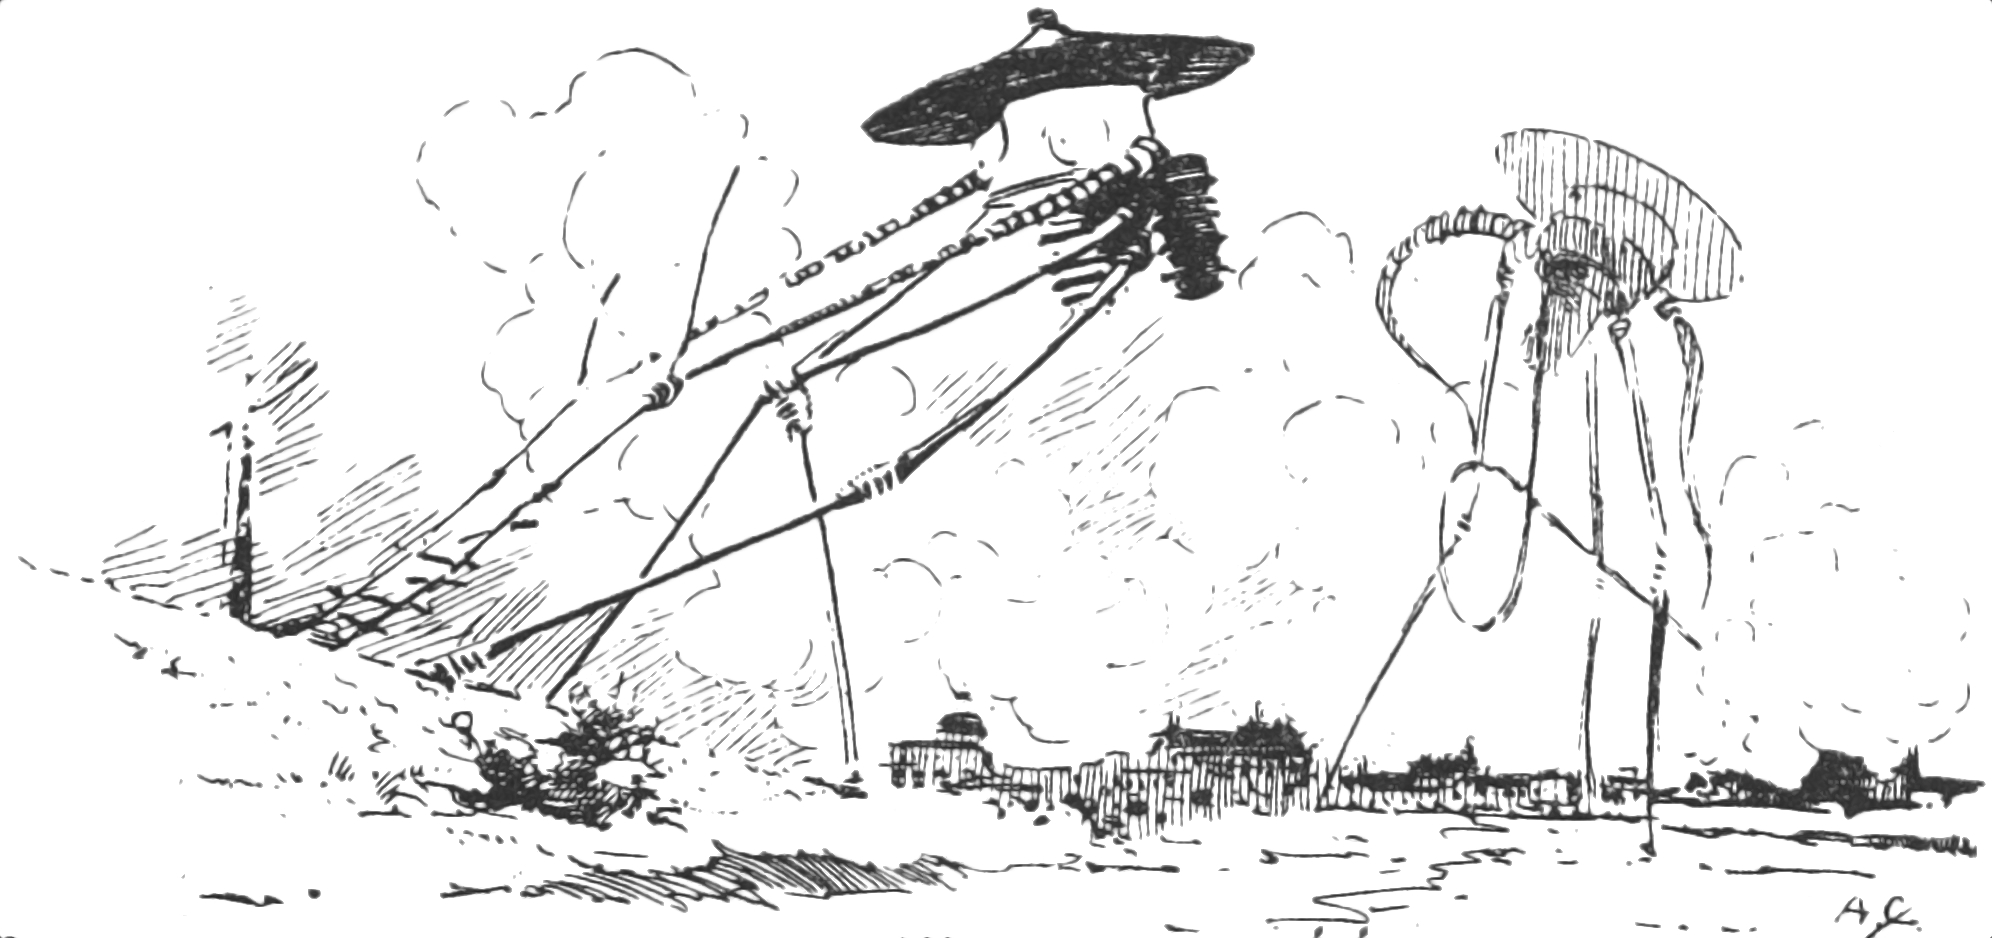
\includegraphics[width=\textwidth]{17tripods}
\end{figure}

Of the falling of the fifth cylinder I have presently to tell. The sixth star fell at Wimbledon.\label{cylinder6} My brother, keeping watch beside the women in the chaise in a meadow, saw the green flash of it far beyond the hills. On Tuesday the little party, still set upon getting across the sea, made its way through the swarming country towards Colchester. The news that the Martians were now in possession of the whole of London was confirmed. They had been seen at Highgate, and even, it was said, at Neasden. But they did not come into my brother's view until the morrow.

That day the scattered multitudes began to realise the urgent need of provisions. As they grew hungry the rights of property ceased to be regarded. Farmers were out to defend their cattle-sheds, granaries, and ripening root crops with arms in their hands. A number of people now, like my brother, had their faces eastward, and there were some desperate souls even going back towards London to get food. These were chiefly people from the northern suburbs, whose knowledge of the Black Smoke came by hearsay. He heard that about half the members of the government had gathered at Birmingham, and that enormous quantities of high explosives were being prepared to be used in automatic mines across the Midland counties.

He was also told that the Midland Railway Company had replaced the desertions of the first day's panic, had resumed traffic, and was running northward trains from St~Albans to relieve the congestion of the home counties. There was also a placard in Chipping Ongar announcing that large stores of flour were available in the northern towns and that within twenty-four hours bread would be distributed among the starving people in the neighbourhood. \label{broexp3}But this intelligence did not deter him from the plan of escape he had formed, and the three pressed eastward all day, and heard no more of the bread distribution than this promise. Nor, as a matter of fact, did anyone else hear more of it. That night fell the seventh star, falling upon Primrose Hill.\label{cylinder7} It fell while Miss Elphinstone was watching, for she took that duty alternately with my brother. She saw it.

On Wednesday the three fugitives—they had passed the night in a field of unripe wheat—reached Chelmsford, \label{broexp4b} and there a body of the inhabitants, calling itself the Committee of Public Supply, seized the pony as provisions, and would give nothing in exchange for it but the promise of a share in it the next day. Here there were rumours of Martians at Epping, and news of the destruction of Waltham Abbey Powder Mills in a vain attempt to blow up one of the invaders.

People were watching for Martians here from the church towers. My brother, very luckily for him as it chanced, preferred to push on at once to the coast rather than wait for food, although all three of them were very hungry. By midday they passed through Tillingham, which, strangely enough, seemed to be quite silent and deserted, save for a few furtive plunderers hunting for food. \label{broexp5a} Near Tillingham they suddenly came in sight of the sea, and the most amazing crowd of shipping of all sorts that it is possible to imagine.

For after the sailors could no longer come up the Thames, they came on to the Essex coast, to Harwich and Walton and Clacton, and afterwards to Foulness and Shoebury, to bring off the people. They lay in a huge sickle-shaped curve that vanished into mist at last towards the Naze. Close inshore was a multitude of fishing smacks—English, Scotch, French, Dutch, and Swedish; steam launches from the Thames, yachts, electric boats; and beyond were ships of larger burden, a multitude of filthy colliers, trim merchantmen, cattle ships, passenger boats, petroleum tanks, ocean tramps, an old white transport even, neat white and grey liners from Southampton and Hamburg; and along the blue coast across the Blackwater my brother could make out dimly a dense swarm of boats chaffering with the people on the beach, a swarm which also extended up the Blackwater almost to Maldon. 

About a couple of miles out lay an ironclad, very low in the water, almost, to my brother's perception, like a water-logged ship. This was the ram \textit{Thunder Child}. \label{broexp6} It was the only warship in sight, but far away to the right over the smooth surface of the sea—for that day there was a dead calm—lay a serpent of black smoke to mark the next ironclads of the Channel Fleet, which hovered in an extended line, steam up and ready for action, across the Thames estuary during the course of the Martian conquest, vigilant and yet powerless to prevent it.

\begin{letter}
	\begin{wrapfigure}{O}{0.6\textwidth}
	\centering
	
\includegraphics[width=0.6\textwidth]{17waterside}
	\end{wrapfigure}
\end{letter}
\begin{a4}
	\begin{figure}[tb]
	\centering
	
\includegraphics[width=.8\linewidth]{17waterside}
	\end{figure}
\end{a4}

At the sight of the sea, Mrs~Elphinstone, in spite of the assurances of her sister-in-law, gave way to panic. She had never been out of England before, she would rather die than trust herself friendless in a foreign country, and so forth. She seemed, poor woman, to imagine that the French and the Martians might prove very similar. She had been growing increasingly hysterical, fearful, and depressed during the two days' journeyings. Her great idea was to return to Stanmore. Things had been always well and safe at Stanmore. They would find George at Stanmore\textellipsis

It was with the greatest difficulty they could get her down to the beach, where presently my brother succeeded in attracting the attention of some men on a paddle steamer from the Thames. They sent a boat and drove a bargain for thirty-six pounds for the three. The steamer was going, these men said, to Ostend.

It was about two o'clock when my brother, having paid their fares at the gangway, found himself safely aboard the steamboat with his charges. There was food aboard, albeit at exorbitant prices, and the three of them contrived to eat a meal on one of the seats forward.

There were already a couple of score of passengers aboard, some of whom had expended their last money in securing a passage, but the captain lay off the Blackwater until five in the afternoon, picking up passengers until the seated decks were even dangerously crowded. He would probably have remained longer had it not been for the sound of guns that began about that hour in the south. As if in answer, the ironclad seaward fired a small gun and hoisted a string of flags. A jet of smoke sprang out of her funnels.

Some of the passengers were of opinion that this firing came from Shoeburyness, until it was noticed that it was growing louder. At the same time, far away in the southeast the masts and upperworks of three ironclads rose one after the other out of the sea, beneath clouds of black smoke. But my brother's attention speedily reverted to the distant firing in the south. He fancied he saw a column of smoke rising out of the distant grey haze.

\begin{figure}[tb!]
\centering

\includegraphics[width=\textwidth]{17boats}
\end{figure}

The little steamer was already flapping her way eastward of the big crescent of shipping, and the low Essex coast was growing blue and hazy, when a Martian appeared, small and faint in the remote distance, advancing along the muddy coast from the direction of Foulness. At that the captain on the bridge swore at the top of his voice with fear and anger at his own delay, and the paddles seemed infected with his terror. Every soul aboard stood at the bulwarks or on the seats of the steamer and stared at that distant shape, higher than the trees or church towers inland, and advancing with a leisurely parody of a human stride.

It was the first Martian my brother had seen, and he stood, more amazed than terrified, watching this Titan advancing deliberately towards the shipping, wading farther and farther into the water as the coast fell away. Then, far away beyond the Crouch, came another, striding over some stunted trees, and then yet another, still farther off, wading deeply through a shiny mudflat that seemed to hang halfway up between sea and sky. They were all stalking seaward, as if to intercept the escape of the multitudinous vessels that were crowded between Foulness and the Naze. In spite of the throbbing exertions of the engines of the little paddle-boat, and the pouring foam that her wheels flung behind her, she receded with terrifying slowness from this ominous advance.

\begin{a4}
\begin{figure}[tb!]
\centering

\includegraphics[width=.7\textwidth]{17fullspeed}
\end{figure}
\end{a4}

% \begin{figure}[p]
% \centering
% 
\includegraphics[width=\linewidth]{17slantingly}
% \caption{Something flat and broad, and very large}
% \end{figure}

\begin{pictures}
\begin{letter}
	\begin{bwbigpic}
		[1.2] 
		{17slantingly} 
		{Something flat and broad, and very large} 
	\end{bwbigpic}
\end{letter}
\begin{a4}
	\begin{bwbigpic}
		[1.1] 
		{17slantingly} 
		{Something flat and broad, and very large} 
	\end{bwbigpic}
\end{a4}
\end{pictures}

Glancing northwestward, my brother saw the large crescent of shipping already writhing with the approaching terror; one ship passing behind another, another coming round from broadside to end on, steamships whistling and giving off volumes of steam, sails being let out, launches rushing hither and thither. He was so fascinated by this and by the creeping danger away to the left that he had no eyes for anything seaward. And then a swift movement of the steamboat (she had suddenly come round to avoid being run down) flung him headlong from the seat upon which he was standing. There was a shouting all about him, a trampling of feet, and a cheer that seemed to be answered faintly. The steamboat lurched and rolled him over upon his hands.

He sprang to his feet and saw to starboard, and not a hundred yards from their heeling, pitching boat, a vast iron bulk like the blade of a plough tearing through the water, tossing it on either side in huge waves of foam that leaped towards the steamer, flinging her paddles helplessly in the air, and then sucking her deck down almost to the waterline.

A douche of spray blinded my brother for a moment. When his eyes were clear again he saw the monster had passed and was rushing landward. Big iron upperworks rose out of this headlong structure, and from that twin funnels projected and spat a smoking blast shot with fire. It was the torpedo ram, \textit{Thunder Child}, steaming headlong, coming to the rescue of the threatened shipping.

\begin{letter}
\begin{figure}[tb!]
\centering

\includegraphics[width=.7\textwidth]{17fullspeed}
\end{figure}
\end{letter}


\begin{pictures} %The \textit{Thunder Child} drove towards them (letter)
	\begin{letter}
		\clearpage
		\begin{tikzpicture}[remember picture, overlay]
			\node (img) at ($(current page.center)+(0.5cm,0cm)$) {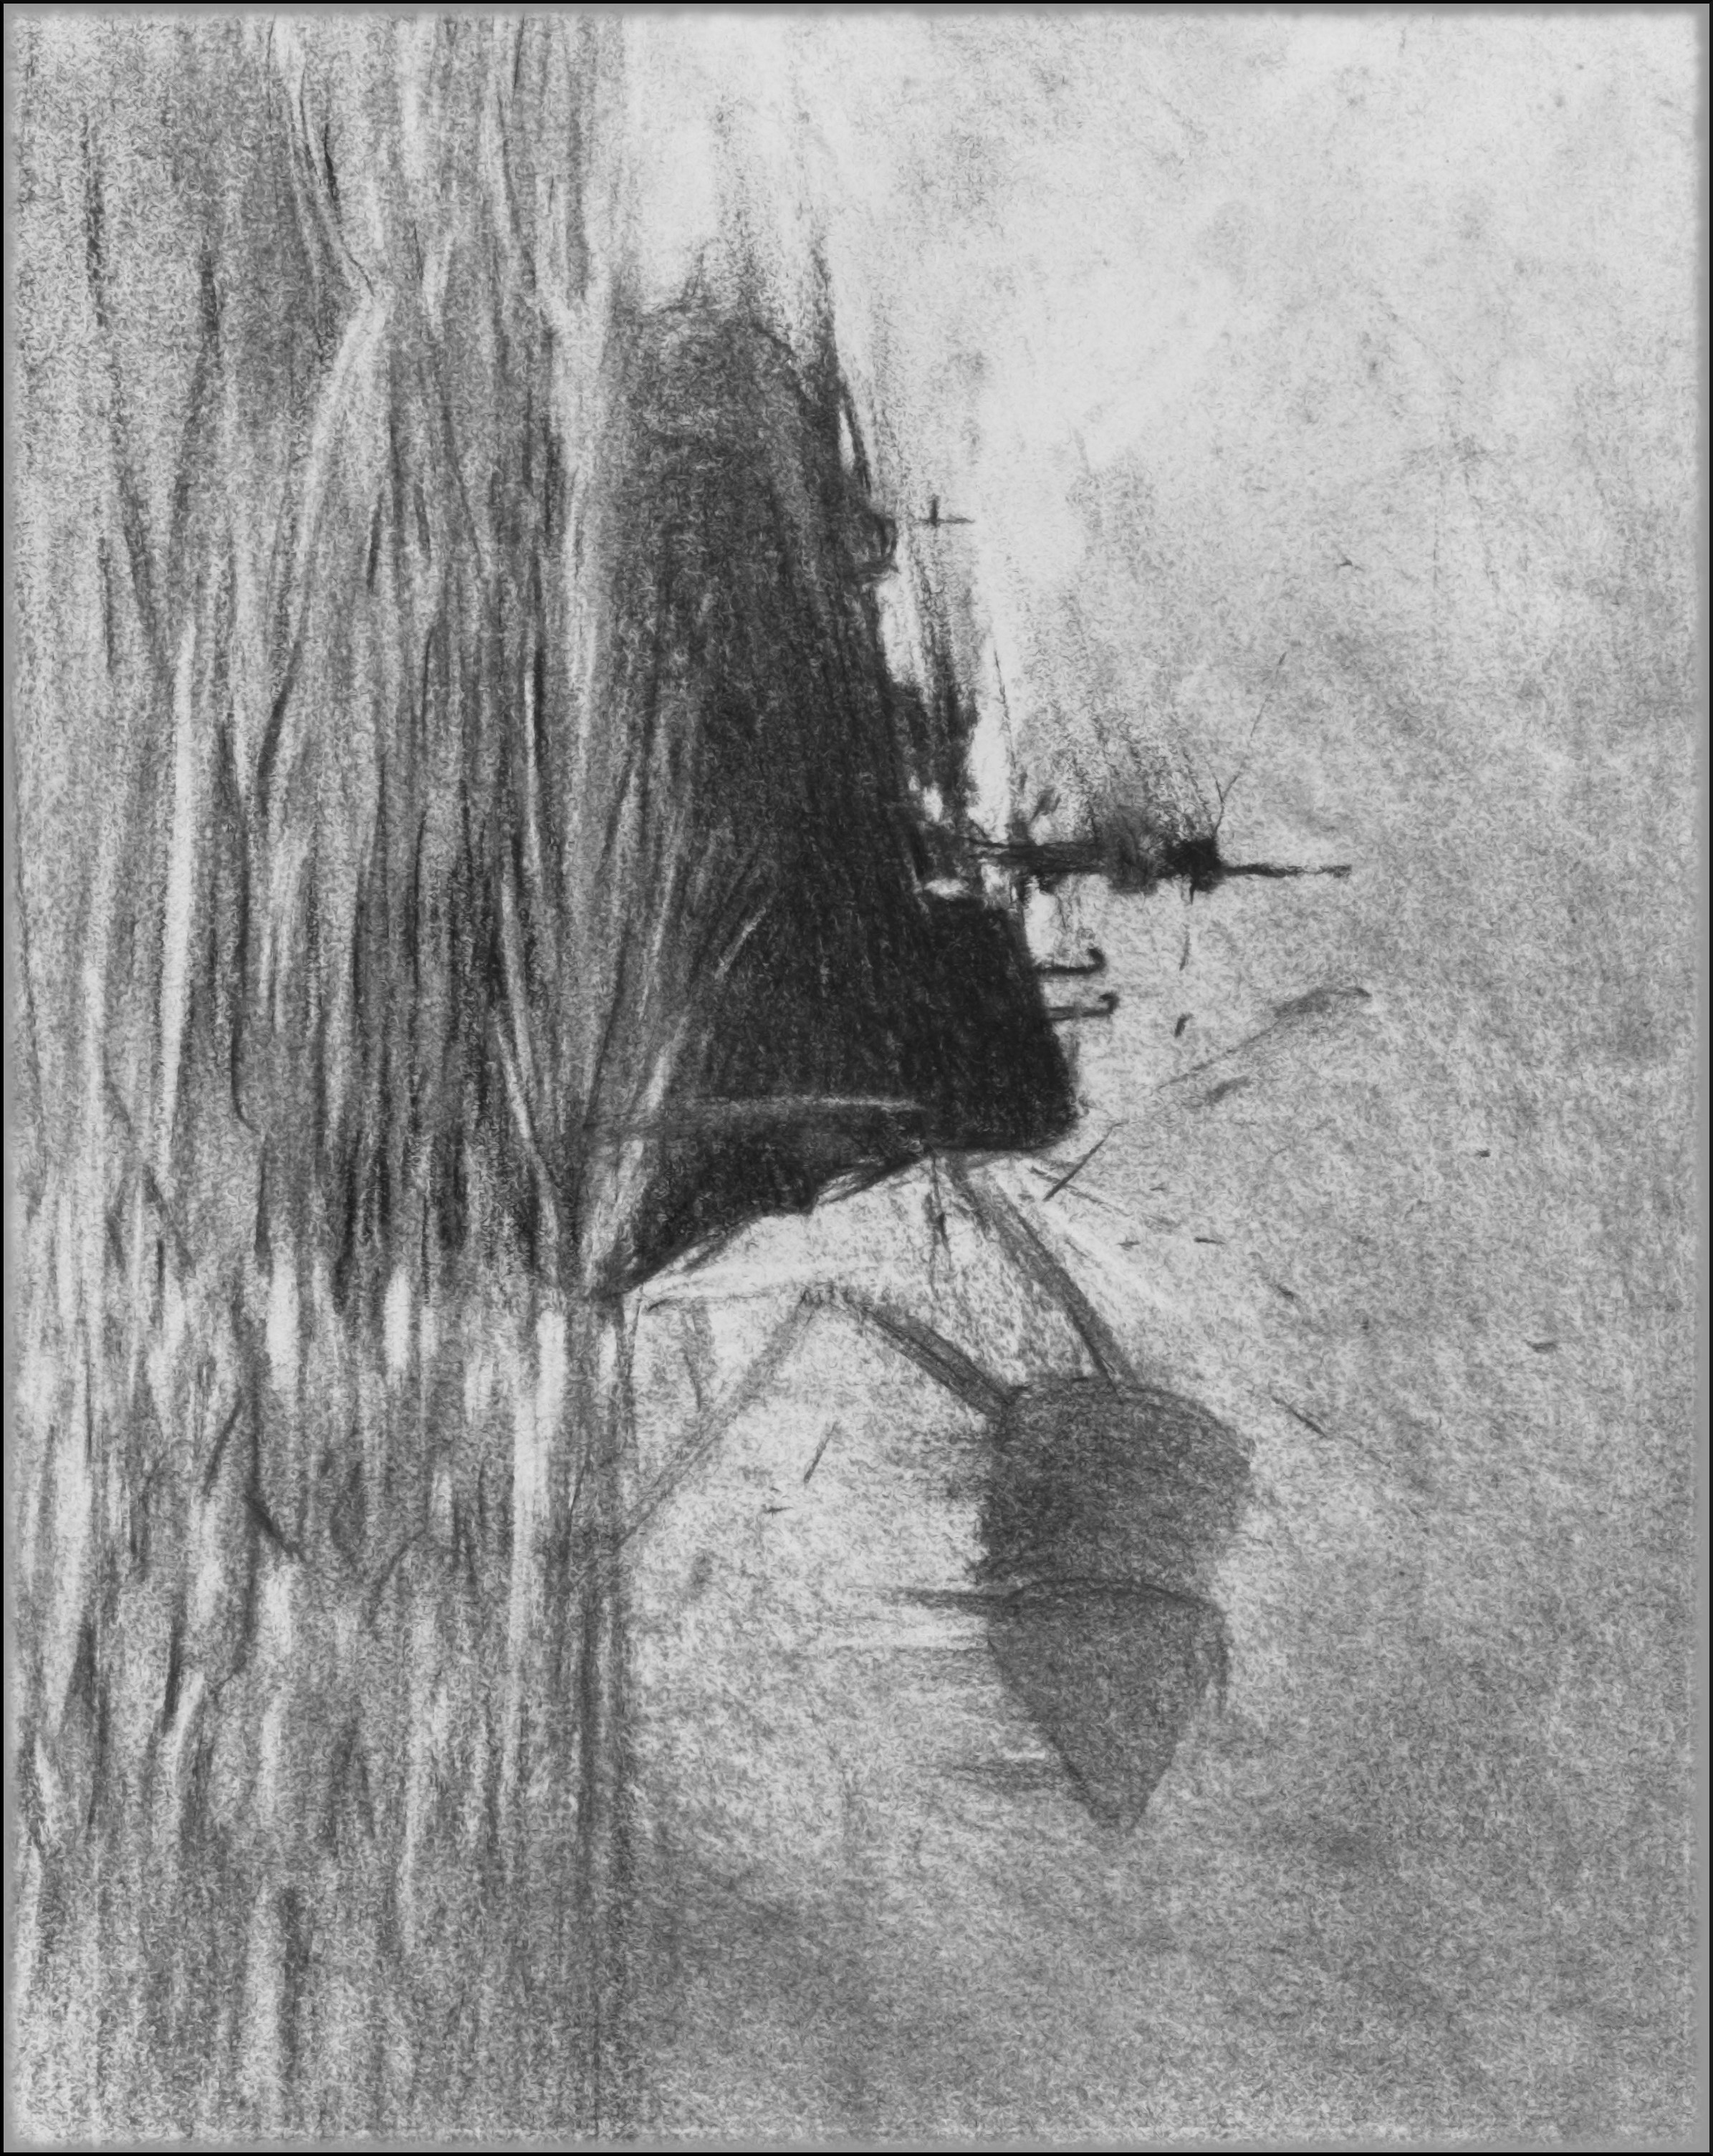
\includegraphics[width=1.15\columnwidth]{17thunderchild}};
			\node[rotate=-90, text width=\textheight, align=center] (caption) at ($(current page.west)+(1cm,0cm)$) {\textsc{The \textit{Thunder Child} simply drove full speed towards them}};

		\end{tikzpicture}
		\thispagestyle{empty}
		\addxcontentsline{lof}{figure}{The \textit{Thunder Child} drove towards them}

		\clearpage
	\end{letter}
\end{pictures}




Keeping his footing on the heaving deck by clutching the bulwarks, my brother looked past this charging leviathan at the Martians again, and he saw the three of them now close together, and standing so far out to sea that their tripod supports were almost entirely submerged. Thus sunken, and seen in remote perspective, they appeared far less formidable than the huge iron bulk in whose wake the steamer was pitching so helplessly. It would seem they were regarding this new antagonist with astonishment. To their intelligence, it may be, the giant was even such another as themselves. The \textit{Thunder Child} fired no gun, but simply drove full speed towards them. It was probably her not firing that enabled her to get so near the enemy as she did. They did not know what to make of her. One shell, and they would have sent her to the bottom forthwith with the Heat-Ray.



She was steaming at such a pace that in a minute she seemed halfway between the steamboat and the Martians—a diminishing black bulk against the receding horizontal expanse of the Essex coast.

Suddenly the foremost Martian lowered his tube and discharged a canister of the black gas at the ironclad. It hit her larboard side and glanced off in an inky jet that rolled away to seaward, an unfolding torrent of Black Smoke, from which the ironclad drove clear. To the watchers from the steamer, low in the water and with the sun in their eyes, it seemed as though she were already among the Martians.

They saw the gaunt figures separating and rising out of the water as they retreated shoreward, and one of them raised the camera-like generator of the Heat-Ray. He held it pointing obliquely downward, and a bank of steam sprang from the water at its touch. It must have driven through the iron of the ship's side like a white-hot iron rod through paper.

A flicker of flame went up through the rising steam, and then the Martian reeled and staggered. In another moment he was cut down, and a great body of water and steam shot high in the air. The guns of the \textit{Thunder Child} sounded through the reek, going off one after the other, and one shot splashed the water high close by the steamer, ricocheted towards the other flying ships to the north, and smashed a smack to matchwood.

But no one heeded that very much. At the sight of the Martian's collapse the captain on the bridge yelled inarticulately, and all the crowding passengers on the steamer's stern shouted together. And then they yelled again. For, surging out beyond the white tumult, drove something long and black, the flames streaming from its middle parts, its ventilators and funnels spouting fire.

She was alive still; the steering gear, it seems, was intact and her engines working. She headed straight for a second Martian, and was within a hundred yards of him when the Heat-Ray came to bear. Then with a violent thud, a blinding flash, her decks, her funnels, leaped upward. The Martian staggered with the violence of her explosion, and in another moment the flaming wreckage, still driving forward with the impetus of its pace, had struck him and crumpled him up like a thing of cardboard. My brother shouted involuntarily. A boiling tumult of steam hid everything again.

»Two!« yelled the captain.

Everyone was shouting. The whole steamer from end to end rang with frantic cheering that was taken up first by one and then by all in the crowding multitude of ships and boats that was driving out to sea.

The steam hung upon the water for many minutes, hiding the third Martian and the coast altogether. And all this time the boat was paddling steadily out to sea and away from the fight; and when at last the confusion cleared, the drifting bank of black vapour intervened, and nothing of the \textit{Thunder Child} could be made out, nor could the third Martian be seen. But the ironclads to seaward were now quite close and standing in towards shore past the steamboat.



The little vessel continued to beat its way seaward, and the ironclads receded slowly towards the coast, which was hidden still by a marbled bank of vapour, part steam, part black gas, eddying and combining in the strangest way. The fleet of refugees was scattering to the northeast; several smacks were sailing between the ironclads and the steamboat. After a time, and before they reached the sinking cloud bank, the warships turned northward, and then abruptly went about and passed into the thickening haze of evening southward. The coast grew faint, and at last indistinguishable amid the low banks of clouds that were gathering about the sinking sun.


\begin{pictures} %The \textit{Thunder Child} drove towards them (a4)
	\begin{a4}
		\clearpage
		\begin{tikzpicture}[remember picture, overlay]
			\node (img) at ($(current page.center)+(0.5cm,0cm)$) {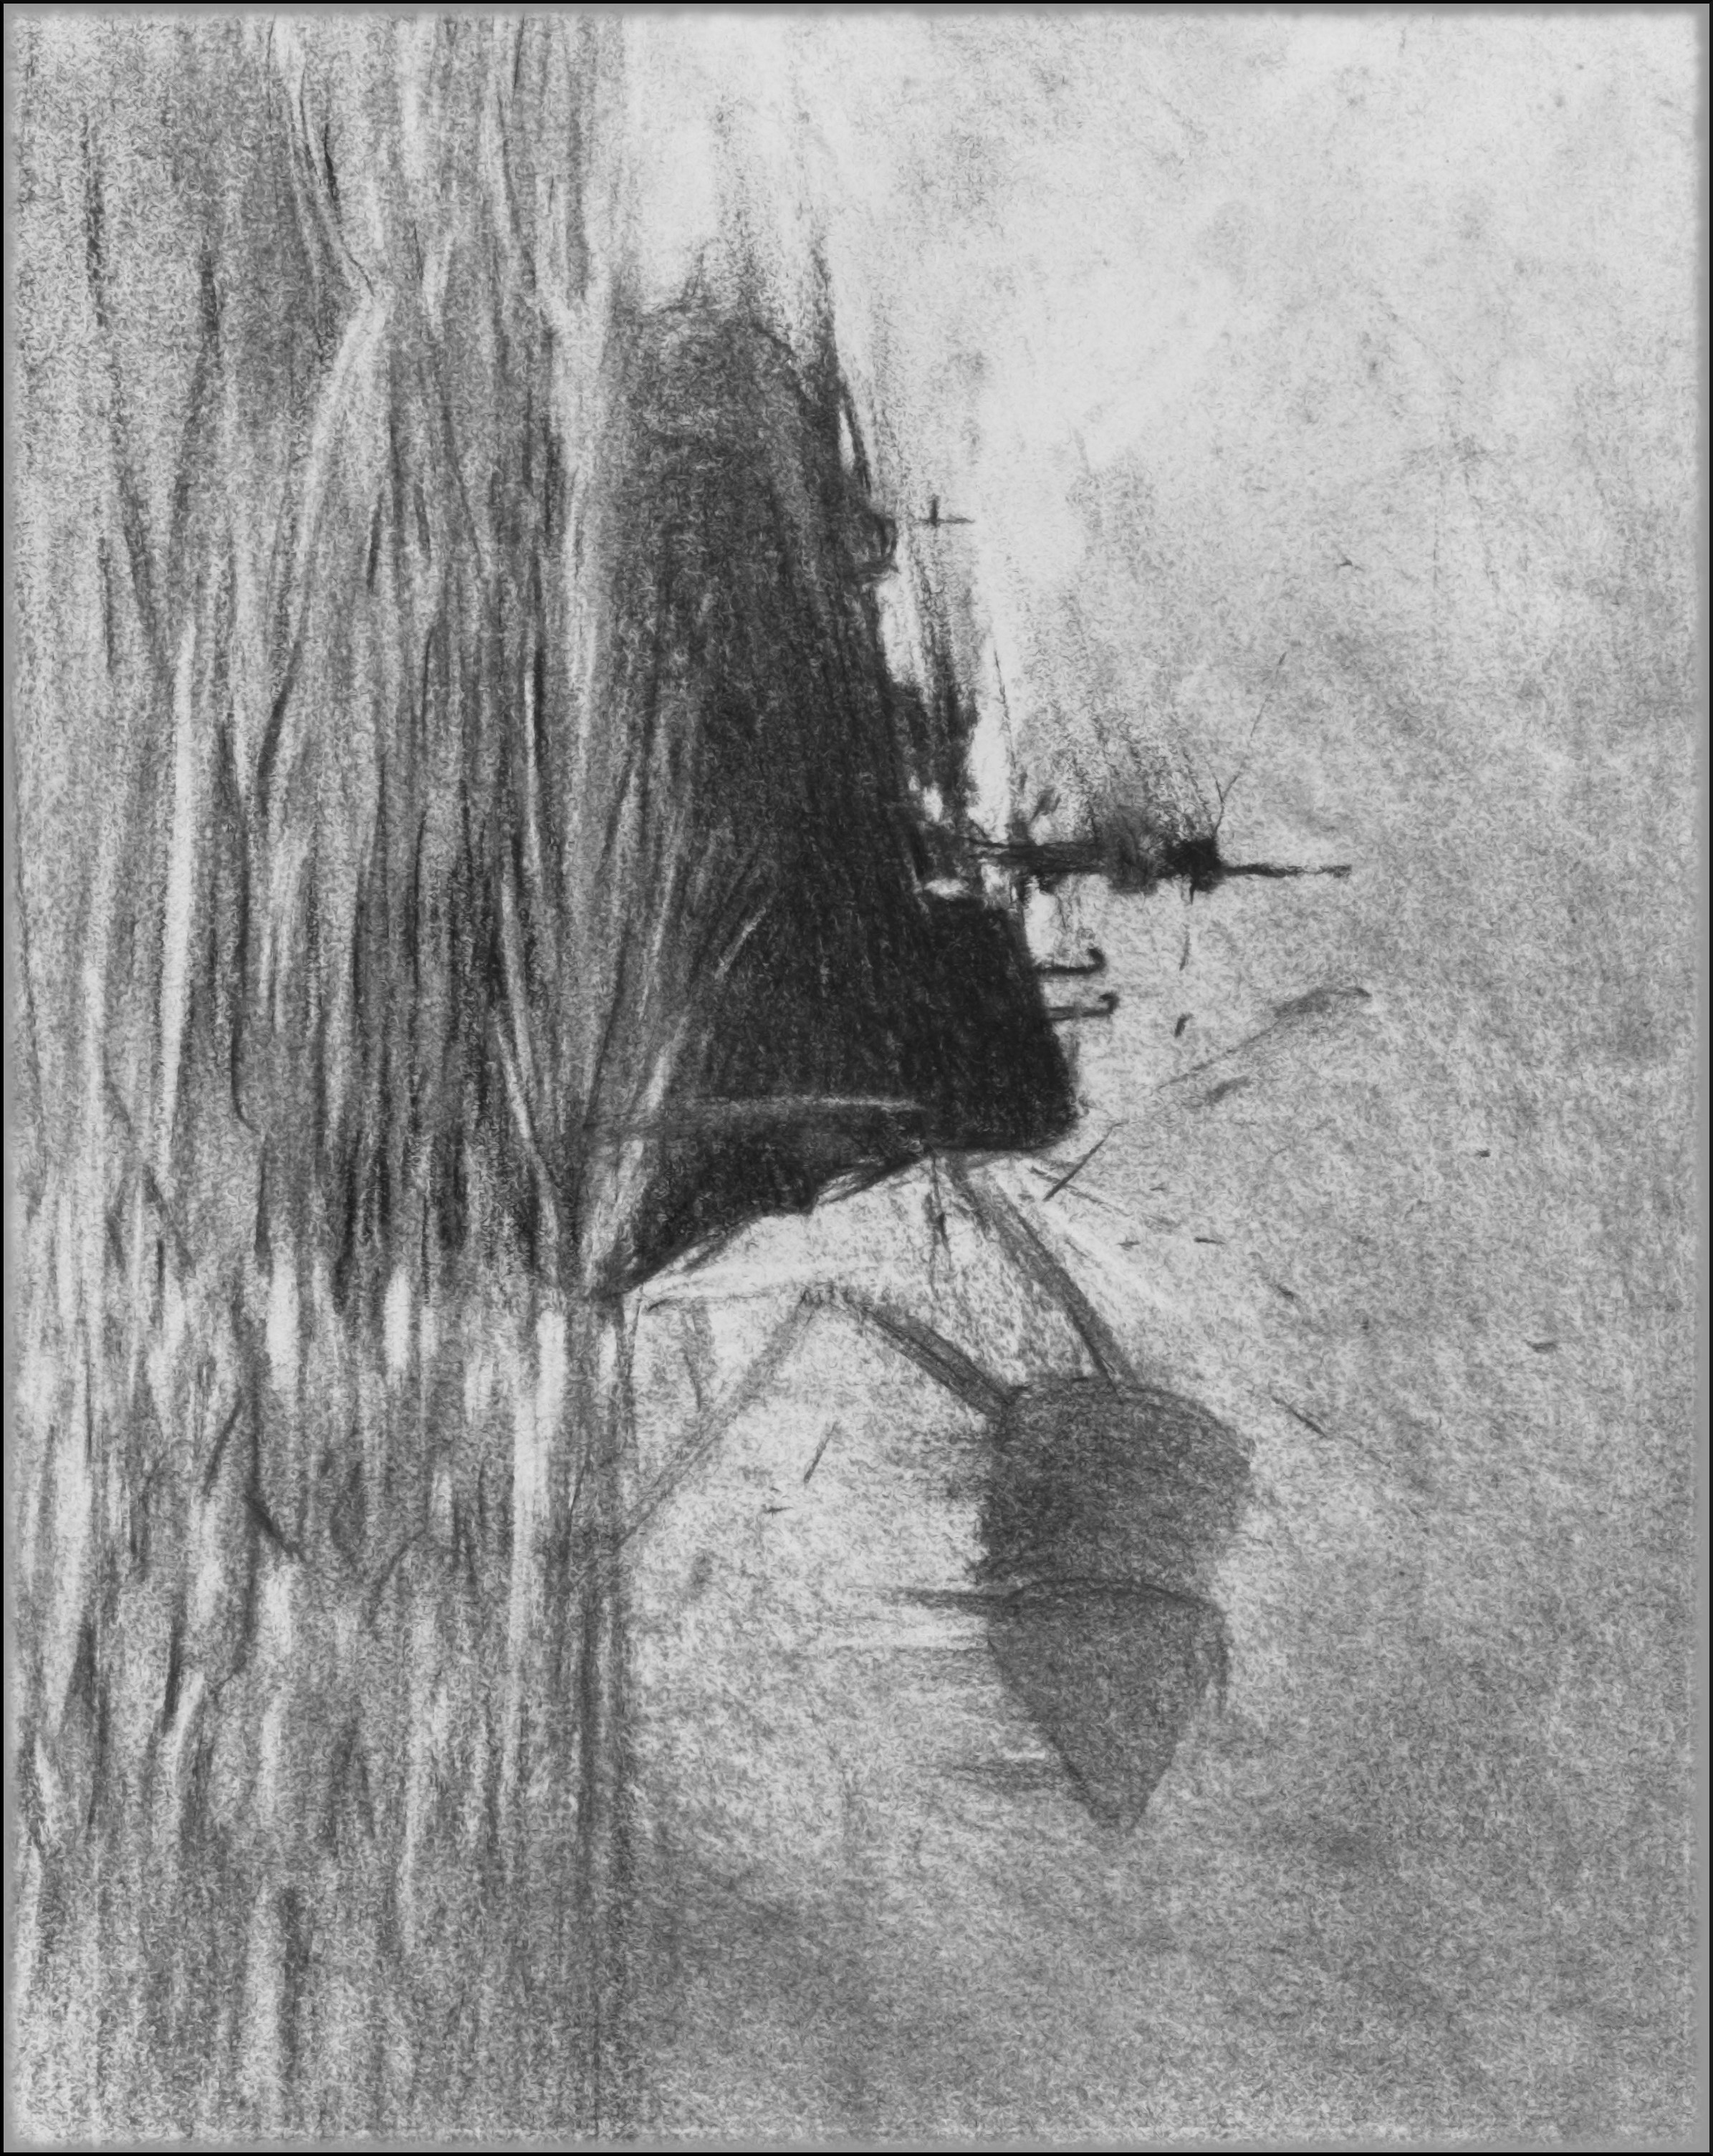
\includegraphics[width=1.15\columnwidth]{17thunderchild}};
			\node[rotate=-90, text width=\textheight, align=center] (caption) at ($(current page.west)+(1cm,0cm)$) {\textsc{The \textit{Thunder Child} simply drove full speed towards them}};

		\end{tikzpicture}
		\thispagestyle{empty}
		\addxcontentsline{lof}{figure}{The \textit{Thunder Child} drove towards them}

		\clearpage
	\end{a4}
\end{pictures}



\begin{a4}
	\begin{wrapfigure}{l}{0.2\textwidth}
		\centering
		
\includegraphics[width=0.2\textwidth]{17snitch}
	\end{wrapfigure}
\end{a4}

Then suddenly out of the golden haze of the sunset came the vibration of guns, and a form of black shadows moving. Everyone struggled to the rail of the steamer and peered into the blinding furnace of the west, but nothing was to be distinguished clearly. A mass of smoke rose slanting and barred the face of the sun. The steamboat throbbed on its way through an interminable suspense.

\begin{letter}
	\begin{wrapfigure}{l}{0.2\textwidth}
		\centering
		
\includegraphics[width=0.2\textwidth]{17snitch}
	\end{wrapfigure}
\end{letter}



The sun sank into grey clouds, the sky flushed and darkened, the evening star trembled into sight. It was deep twilight when the captain cried out and pointed. My brother strained his eyes. Something rushed up into the sky out of the greyness—rushed slantingly upward and very swiftly into the luminous clearness above the clouds in the western sky; something flat and broad, and very large, that swept round in a vast curve, grew smaller, sank slowly, and vanished again into the grey mystery of the night. And as it flew it rained down darkness upon the land.


\begin{a4}
	\begin{figure}[b!]
		\centering
		
\includegraphics[width=.7\linewidth]{17tailpiece}
	\end{figure}
\end{a4}

\begin{letter}
	\begin{figure}[b!]
		\centering
		
\includegraphics[width=.8\linewidth]{17tailpiece}
	\end{figure}
\end{letter}




